\documentclass[12pt,a4paper]{article}
\usepackage[ngerman]{babel}
\usepackage[utf8]{inputenc}
\usepackage[unicode=true,bookmarks=false,bookmarksopen=true]{hyperref}

\usepackage{xcolor}
\usepackage{graphicx}
\usepackage{tikz}

\def\checkmark{\tikz\fill[scale=0.4](0,.35) -- (.25,0) -- (1,.7) -- (.25,.15) -- cycle;}

\title{ORES Preparation III}
\author{Tom Gülenman}
\begin{document}
\maketitle
\textit{Disclaimer: No guarantee for the correctness of information / explanations / sources is given.}\\
\section*{Goals}
\begin{enumerate}
\item Check out IRC Channel \checkmark
\item Read towardsdatascience article \checkmark
\item Research the model item quality \checkmark
\item Study pipeline definition $\times$
\item Take a look at LIME + Machine Learning \checkmark
\item Understand and describe all parameters $\sim$ mostly
\begin{itemize}
\item Get in touch on IRC and ask if there is a list of all parameters (and what match\_rate means?) \checkmark
\end{itemize}
\item Open repository on Github to document the research \checkmark
\item Research $\sim$
\begin{enumerate}
\item In what other cases than confusion matrices are those parameters explained?
\item Are there already visualizations of some of these parameters in any contexts?
\item Are there any applications, where I can filter for these parameters $\rightarrow$ visualizations or just about anything?
\end{enumerate}
\end{enumerate}
\section{IRC Channel}
Link: \href{https://webchat.freenode.net/?channels=#wikimedia-ai}{IRC Freenode \#wikimedia-ai}
\section{Beyond Accuracy: Precision and Recall}
Link: \href{https://towardsdatascience.com/beyond-accuracy-precision-and-recall-3da06bea9f6c}{Towards Data Science}
\begin{itemize}
\item Classification problems: is passenger a terrorist?
\item Positive class is way smaller than negative $\rightarrow$ accuracy is not a good measure for model performance (for example 99\%) models aren't good enough
\item Focus on identifying positive cases:
\item \colorbox{cyan}{\textbf{Recall}}: Ability of model to find all relevant cases within dataset
\item Recall $= \frac{\texttt{true positives}}{\texttt{true positives} + \texttt{false negatives}}$ \[= \frac{\texttt{terrorists correctly ident.}}{\texttt{terr.corr.ident.}+\texttt{terrorists incorrectly labeled as not terrorists}}\]
\begin{description}
\item Labeling everyone as terrorist $\rightarrow$ \textbf{recall} = 1.0
\item But low \textbf{precision}!
\end{description}
\item \colorbox{cyan}{\textbf{Precision}}: Ability of model to find only relevant cases within dataset
\item Precision $= \frac{\texttt{true positives}}{\texttt{true positives} + \texttt{false positives}}$ \[ = \frac{\texttt{terrorists correctly ident.}}{\texttt{terr.corr.ident.}+\texttt{individuals incorrectly labeled as terrorists}}\]
\item Other hypoth. model: only identify one single terrorist correctly
\begin{description}
\item \textbf{Recall} really low but:
\item \textbf{Precision} = 1.0
\end{description}
\item \colorbox{cyan}{Key learning}: Increasing \textbf{recall} decreases \textbf{precision} and vice versa
\end{itemize}
\subsection{Combining Precision and Recall}
\begin{itemize}
\item There are cases in which we want to maximize one of those 2 parameters
\item But if we want an optimal combination: \colorbox{cyan}{\textbf{F1}-score}, the harmonic mean of precision and recall
\item \textbf{F1} $=2*\frac{\texttt{precision} * \texttt{recall}}{\texttt{precision}+\texttt{recall}}$
\item Better than using simple average because it punishes extreme values:
\begin{description}
\item Classifier with precision 1.0 and recall 0.0 has average of 0.5, but \textbf{F1} = 0.0
\item Optimal balance of \textbf{precision} and \textbf{recall} $\Rightarrow$ maximize \textbf{F1}
\end{description}
\end{itemize}
\subsection{Visualizing Precision and Recall}
\begin{itemize}
\item Confusion Matrix:\\
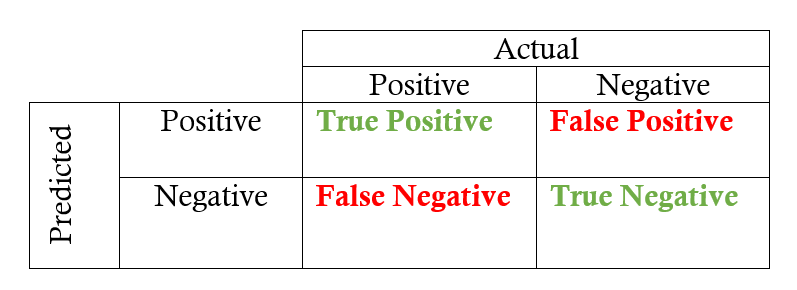
\includegraphics[scale=.3]{resources/3/confusionMatrix}
\item ROC curve (Receiver Operating Characteristic):
\begin{itemize}
\item Definition: plots the true positive rate (TPR) versus the false positive rate (FPR) as a function of the model’s threshold for classifying a positive
\item True Positive Rate (=Recall): $\frac{\texttt{TP}}{\texttt{TP}+\texttt{FN}}$
\item False Positive Rate: $\frac{\texttt{FP}}{\texttt{FP}+\texttt{TN}}$
\begin{description}
\item \colorbox{cyan}{\textbf{tpr}}: the portion, of all positive data, that was predicted as positive
\item \textbf{fpr}: the portion, of all negative data, that was predicted as positive
\end{description}
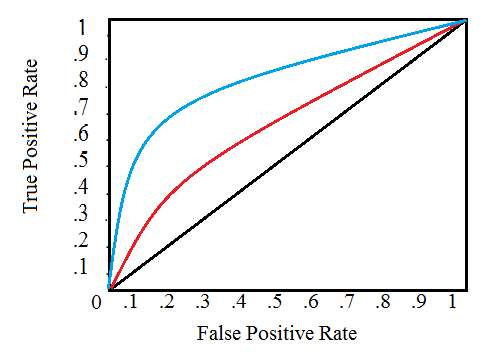
\includegraphics[scale=0.5]{resources/3/ROCcurve}
\begin{description}
\item Bottom left: Decision threshold = 1.0 $\Rightarrow$ all data is predicted as false $\rightarrow$ tpr = fpr = 0.0
\item Top right: \colorbox{cyan}{Decision threshold} = 0.0 $\Rightarrow$ all data is predicted as positive $\rightarrow$ tpr = fpr = 1.0
\item \colorbox{yellow}{Question:} \textbf{tpr} = 1.0 also works if all positive data is predicted as positive and all the negative data is predicted as negative, but then tpr$=1.0\neq $fpr$=0.0$... (How is this graphic still correct?)
\end{description}
\item We can quantify ROC curve by calculating the area under the curve (AUC): metric between 0 and 1
\begin{description}
\item AUC of blue curve $>$ AUC of red curve $\Rightarrow$ blue classifier is better at achieving blend of precision and recall
\item Random classifier (black line) has AUC of 0.5
\end{description}
\end{itemize}
\end{itemize}
\subsection{Example Application}
\textit{Definitely worth checking out in the article itself.} Amongst other things: how to calculate F1 from confusion matrix
\subsection{Conclusion}
\textit{Accuracy is not always the most useful metric.} Instead, \textbf{recall}, \textbf{precision}, \textbf{F1} and \textbf{ROC} help us assess classifications in smarter ways in some contexts.
\section{Itemquality}
\begin{itemize}
\item We are looking into the \textit{itemquality} model in the wikidatawiki context, containing the \textit{damaging}-, \textit{goodfaith}- and \textit{itemquality}-model. 
\item Also, Wikidata is the central storage for structured data of many Wikimedia projects (including Wikipedia).
\item \href{https://www.wikidata.org/wiki/Wikidata:Introduction}{Wikidata Wiki link}: ``The Wikidata repository consists mainly of items, each one having a label, a description and any number of aliases. Items are uniquely identified by a Q followed by a number, such as Douglas Adams'': \href{https://www.wikidata.org/wiki/Q42}{42}
\item Now the purpose of the itemquality model becomes clear: rate the quality of said items
\end{itemize}
%
%
\section{Pipeline definition \colorbox{red}{?}}
\begin{itemize}
\item \href{https://github.com/wikimedia/articlequality/blob/master/Makefile#L572-L651}{Github Link}
\item This line in particular determines which features are used: \href{https://github.com/wikimedia/articlequality/blob/master/Makefile#L637}{Github Link}
\item Constructing the feature list, culminating in: \href{https://github.com/wikimedia/articlequality/blob/master/articlequality/feature_lists/wikidatawiki.py#L166}{Github Link}
\end{itemize}
%
%
\section{LIME and Machine Learning}
\begin{itemize}
\item Link: \href{https://en.wikipedia.org/wiki/Lime_(software)}{\textbf{lime}, a unit testing and functional testing framework}
\item Adam Wight's Lime Sandbox: \href{https://github.com/adamwight/ores-lime/}{Github link}
\begin{description}
\item $\rightarrow$ Take a look at ``Explain draft topic.ipynb'':
\item Use Lime to explain the scores a drafttopic (see: \url{https://en.wikipedia.org/?oldid=42344094}) got
\item The result will be ``[('Culture.Language and literature', 0.5791824638170249),
 ('Geography.Countries', 0.3864267805975978), ...]''
\item After specifying a few parameters for the Lime explainer, it can be used to explain the scoring; results will look like this: 
\item 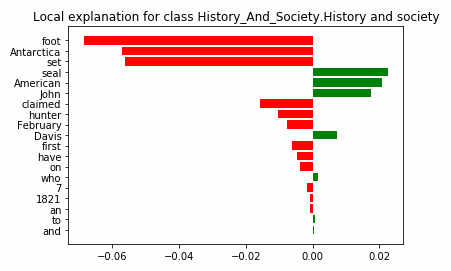
\includegraphics[scale=0.7]{resources/3/limeExplainer}
\end{description}
\end{itemize}
\section{Crucial Metrics}
%This section will also be made available as an extra document
\textit{As described in this article on Towards Data Science} (\href{https://towardsdatascience.com/beyond-accuracy-precision-and-recall-3da06bea9f6c}{Link}
), \textit{the right metrics for classification tasks heavily depend on the context. Let's take a look at possible parameters/metrics to use in ORES API queries.}
\\
Keep in mind the confusion matrix:\\
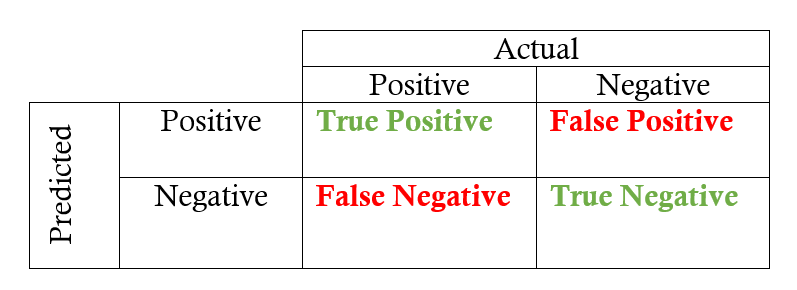
\includegraphics[scale=0.4]{resources/3/confusionMatrix}\\
Or in another format:\\
\includegraphics[scale=0.4]{resources/3/confusionCircle}
\begin{description}
\item Note that the colors of all parts of the circle are always a mix of two colors from the legend on the right.
\end{description}
The following subsections describe interesting metrics, notably in the wikidatawiki context and, more precisely, itemquality model, and will be defined and described with the help of the already mentioned sources, not only from this file, but from other files within the repository as well. 
\subsection{Recall}
\begin{itemize}
\item Recall ($\equiv$ True Positive Rate) is defined as the ability of a model to find all relevant cases within the dataset.
\item Or: the portion, of all actual positive data, that was labeled as positive
\item In other words Recall $= \frac{\texttt{TP}}{\texttt{TP} + \texttt{FN}}$
\item Again in other words $ =\frac{\texttt{correctly\_labeled\_as\_positives}}{\texttt{actual\_positives}}$
\item $=\frac{
\includegraphics[scale=0.1]{resources/3/confusionCircleTP}}{
\includegraphics[scale=0.1]{resources/3/confusionCircleTP+FN}}$
\end{itemize}
\subsection{Precision}
\begin{itemize}
\item Ability of the model to find only relevant cases within the dataset
\item The portion, of all as ``positive'' labeled data, that is actually positive
\item $= \frac{\texttt{TP}}{\texttt{TP} + \texttt{FP}}$
\item $= \frac{\texttt{correctly\_labeled\_as\_positives}}{\texttt{all\_labeled\_as\_positive}}$
\item $=\frac{
\includegraphics[scale=0.1]{resources/3/confusionCircleTP}}{
\includegraphics[scale=0.1]{resources/3/confusionCircleTP+FP}}$
\end{itemize}
\subsection*{Recall vs Precision}
When increasing one of these two, the other one naturally decreases. For an intuitive example, let's take a look at \href{https://research.google.com/bigpicture/attacking-discrimination-in-ml/}{Google's Loan Threshold Simulation}:\\
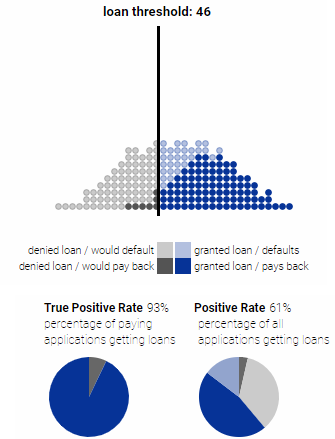
\includegraphics[scale=0.7]{resources/3/loanML3}\\
\begin{description}
\item The dark grey / dark blue dots, representing clients that would actually pay back their loan, are more and more included ($\rightarrow$ given loans) if we move the threshold further to the left.
\item But so are clients that would not. Thus moving the threshold to the left increases the \textbf{recall} (\textbf{tpr}) but decreases the \textbf{precision} and vice versa when moving to the right.
\end{description}
\subsection{f1}
\begin{itemize}
\item F1-Score: The optimal combination of recall and precision: the harmonic mean of the two
\item \textbf{f1} $=2*\frac{\texttt{precision} * \texttt{recall}}{\texttt{precision}+\texttt{recall}}$
\item Note: harmonic mean is used instead of average to punish extreme values (e.g. precision 1.0 and recall 0.0 $\rightarrow$ average 0.5, but F1 $= 0$)
\end{itemize}
\subsection{fpr}
\begin{itemize}
\item We have already mentioned the \textbf{TPR}, now, the false positive rate (\textbf{FPR}) is the probability of a false alarm
\item The portion, of all negatives, that were labeled as positives ($\rightarrow$ false positives):
\item \textbf{fpr} $= \frac{\texttt{FP}}{\texttt{FP} + \texttt{TN}}$ 
\end{itemize}
\subsection{roc\_auc}
\begin{itemize}
\item Summarize the performance of a classifier over all possible thresholds
\item The receiver operating characteristic (ROC) curve plots the TPR versus FPR as a function of the model’s threshold for classifying a positive
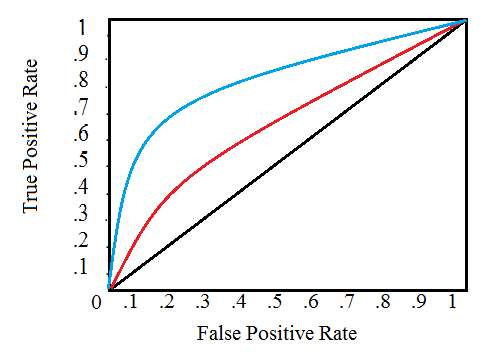
\includegraphics[scale=0.5]{resources/3/ROCcurve}
\begin{description}
\item Two classifiers are shown, one in blue, one in red. The black line is a random classifier.
\item Keep in mind that on the \colorbox{green}{X-} and \colorbox{orange}{Y-axis} we have the portion, of all \colorbox{green}{negative} and of all \colorbox{orange}{positive} data, respectively, that was predicted as positive
\item As we increase the threshold we include fewer and fewer data (also data labeled as positive), thus moving down to the bottom left ($\rightarrow$ decision threshold = 1.0) on the corresponding curve; top right $\rightarrow$ threshold = 0.0
\item That means at the top right corner all data is predicted as positive and in the bottom left corner all data is predicted as negative
\end{description}
\item Now, to evaluate / quantify a given ROC, we calculate the area under the curve (\textbf{AUC})
\item The AUC is a metric between 0 and 1, where higher values signify better capability of achieving a blend of precision and recall (since a higher peaking curve means higher \textbf{tpr})
\item Note: the random classifier will achieve an AUC of $0.5$.
\end{itemize}
\subsection{pr\_auc}
\begin{itemize}
\item This one stands for \textbf{Precision Recall AUC} (see: \url{http://www.chioka.in/differences-between-roc-auc-and-pr-auc/})
\item Sample PR-curve: 
\begin{description}
\item 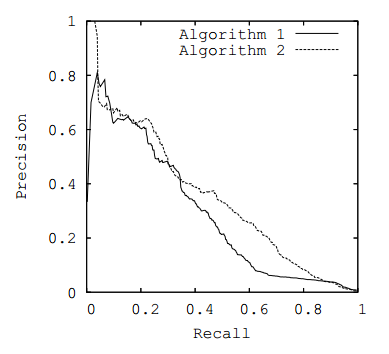
\includegraphics[scale=0.7]{resources/3/PRcurve}
\item Instead of the top left corner for the ROC-curve, here, we want to be in the top right corner for our classifier to be perfect
\end{description}
\item \textbf{pr\_auc} is, as expected, the area under the PR-curve. The higher its value, the better the model 
\end{itemize}
\subsection{roc\_auc vs pr\_auc}
see: \url{https://www.kaggle.com/general/7517}
\begin{itemize}
\item In short, if the class imbalance problem exists, \textbf{pr\_auc} is more appropriate than \textbf{roc\_auc}
\begin{description}
\item If TNs are not meaningful to the problem or there are a lot more negatives than positives, \textbf{pr\_auc} is the way to go (it does not account for TNs).
\end{description}
\item Intuitive explanation: 
\begin{itemize}
\item If the model needs to perform equally on the positive and negative class $\rightarrow$ \textbf{roc\_auc}
\item If it's not interesting how the model performs on negative class $\rightarrow$ \textbf{pr\_auc} (example: detecting cancer; find all positives and make sure they're correct!)
\end{itemize}
\end{itemize}
\subsection{accuracy}
\begin{itemize}
\item \textbf{accuracy}$= \frac{\texttt{TP}+\texttt{TN}}{\texttt{Total}} =\frac{
\includegraphics[scale=0.1]{resources/3/confusionCircleTP+TN}}{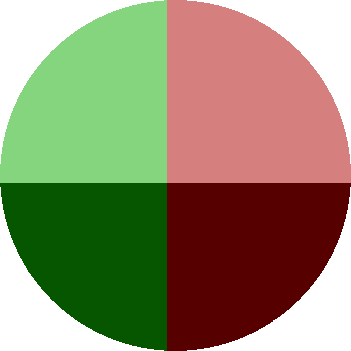
\includegraphics[scale=0.1]{resources/3/confusionCircleTotal}}$
\end{itemize}
\subsection{match\_rate}
\begin{itemize}
\item ``The proportion of observations matched/not-matched''
\item \textbf{match\_rate} $=\frac{\texttt{TP}+\texttt{FP}}{\texttt{Total}}=\frac{
\includegraphics[scale=0.1]{resources/3/confusionCircleTP+FP}}{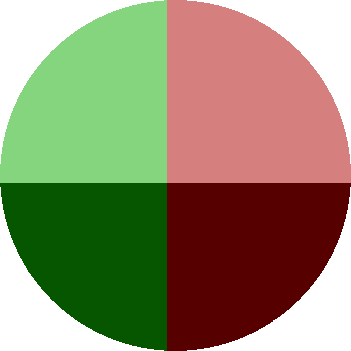
\includegraphics[scale=0.1]{resources/3/confusionCircleTotal}}$
\end{itemize}
\subsection{filter\_rate}
\begin{itemize}
\item ``The proportion of observations filtered/not-filtered'' (?)
\item \textbf{filter\_rate} $=1-\texttt{match\_rate}$
\item $=\frac{\texttt{TN}+\texttt{FN}}{\texttt{Total}} = \frac{
\includegraphics[scale=0.1]{resources/3/confusionCircleTN+FN}}{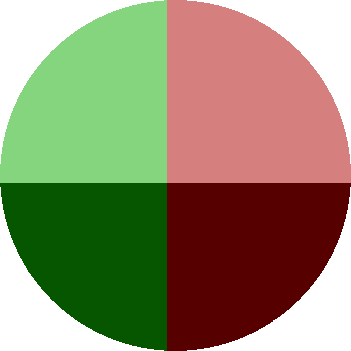
\includegraphics[scale=0.1]{resources/3/confusionCircleTotal}}$
\end{itemize}
\subsection{!$<$metric$>$}
\begin{itemize}
\item Any $<$metric$>$ with an exclamation mark is the same metric for the negative class
\item e.g. recall $= \frac{\texttt{TP}}{\texttt{TP} + \texttt{FN}} \Rightarrow$ \textbf{!}recall  $= \frac{\texttt{TN}}{\texttt{TN} + \texttt{FP}}$
\item Example usage: find all items that are not ``E'' class $\rightarrow$ look at \textbf{!}recall for ``E'' class.
\end{itemize}
\subsubsection{Existing !$<$metric$>$s}
\begin{itemize}
\item !f1
\item !precision
\item !recall
\end{itemize}
\section{Github Repository}
To be found at:\\
\url{https://github.com/tguelenman/OresCustomDocumentation}

\section{Research}
\subsection{Confused Pie Plots}
source:\\
\url{http://www.dietergalea.com/confusion-matrices-alternative/}\\
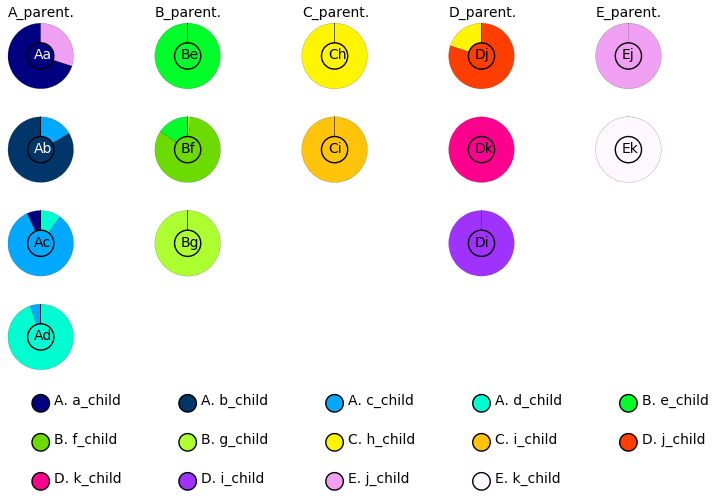
\includegraphics[scale=0.6]{resources/3/confusedPiePlots}
\begin{description}
\item Good for multi-class classification with a lot of classes (or probably even good for 5 or more)
\end{description}
\begin{itemize}
\item Inner ellipse: show the expected target class
\item Outer ellipse: predicted classes
\item Rows here: child nodes
\item Maybe applicable for itemquality $\rightarrow$ multiple classes... somehow?
\item Python code available: check on website linked above or on Github:\\ \url{https://github.com/dterg/confused-pie-plots}
\end{itemize}
%%%
%%%
%%%

\section*{Questions}
\begin{itemize}
\item \colorbox{yellow}{Q:} What's the relation between F1 and ROC\_AUC? Article describes them as: F1: ``If we want to create a balanced classification model with the optimal balance of recall and precision, then we try to maximize the F1 score.''; ROC\_AUC: ``AUC ... will be greater ... meaning ... better at achieving a blend of precision and recall.''
\begin{description}
\item \colorbox{orange}{A:} F1 is used for one threshold value, ROC\_AUC summarizes the performance of a model for all thresholds
\end{description}
%
\end{itemize}
\end{document}
%check out FAT conference for research